\documentclass[a4paper, titlepage]{article}

\usepackage[english]{babel}
\usepackage[utf8x]{inputenc}
\usepackage{amsmath}
\usepackage{amsfonts}
\usepackage{amssymb}
\usepackage{graphicx}
\usepackage{fullpage}
\usepackage{parskip}
\usepackage{setspace}
\usepackage[justification=centering]{caption}

\linespread{1.1}

\title{Visualisation AppStore \\ \vspace{10pt}
\textit{\large Integrated platform for visualistion submission, scheduling and visualisation wall playout} \\ \vspace*{-5pt}
\textit{\large Commissioned by Imperial Data Science Institute}}

\author{Andrew Higginson\\ Bryan Liu \\ Emma Hulme \\ Jia Guang Choo \\
        Thomas Taylor-Hall \\ Timothy van Bremen \\\\ \textit{Supervised by:} \\
        Prof. Yi-ke Guo \\ Dr. David Birch}

\date{January 2015}

\begin{document}
\maketitle


\newpage
\pagenumbering{roman}
% -- Executive Summary
\Large
\textbf{Executive Summary}

\normalsize




% ---

\newpage
% -- Table of Contents
\tableofcontents
\listoffigures
\listoftables
% ---


\newpage
\pagenumbering{arabic}
\section{Introduction}

\subsection{Motivation}

\subsection{Objectives}

\subsubsection{Visualisation Submission}


\subsubsection{Quality Control and Moderation}


\subsubsection{``AppStore'' for Visualisation}


\subsubsection{Scheduling \& Featuring of Visualisation Display}


\subsubsection{Video Walls Playout Software}



\subsection{Achievements}

\newpage
\section{Project Management}

\subsection{Task Estimation}
The group is acutely aware that with Computing examinations being held at the
end of term, we could only practically carry out development work until the
first week of December. Furthermore, commitments in other courses mean that 
each team member is only able to devote around 16-20 hours per week to
the project. As a group, we have allowed some leeway for each task in case we run into technical errors. If this is the case, we will communicate between the group and come up with a solution if necessary.

In light of these constraints, we have decided to commit to the following:
\begin{enumerate}
  \item \textbf{To maintain a one-week iteration}: this allows the development team to
        obtain maximum possible feedback from the client/supervisor.
  \item \textbf{To strictly adhere to the original project scope}: while we believe the
        current scope is manageable, we would reject time-consuming items which
        are out of scope before a minimal working system is implemented.
\end{enumerate}


\begin{figure}[h]
  \centering
%    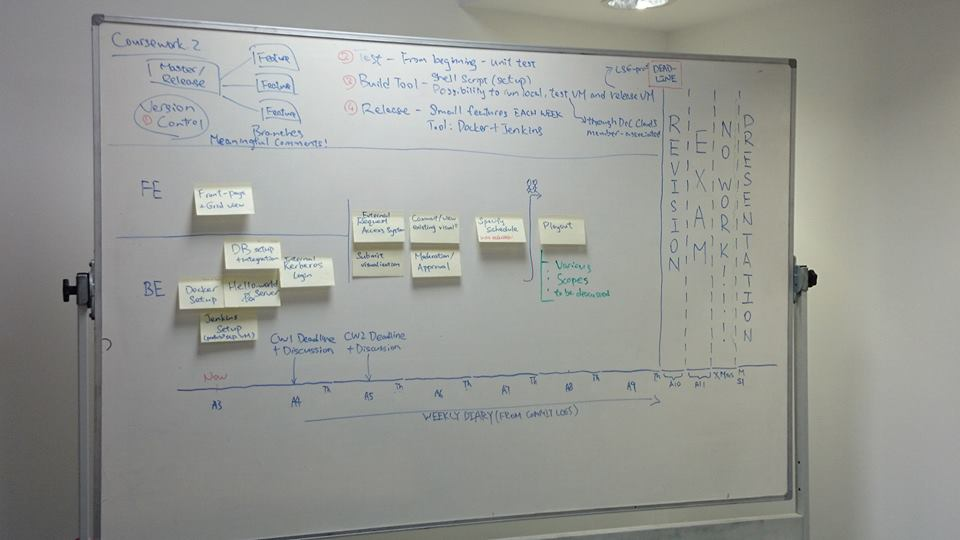
\includegraphics[width = 0.99\textwidth]{./planning/timeline.jpg}
   
  \caption{Project plan with timeline}
  \label{fig:timeline}
\end{figure}


\begin{table}[h]
  \begin{tabular}{c | c | c | c }
    \textbf{Academic Week} & 3 \& 4 (ending 30/10) & 5 (ending 6/11) \\
    \textbf{Iteration/Sprint} & 1 & 2 \\ \hline
    \textbf{Tasks} & Front-page + grid view (FE) & Access request for externals \\
          & Docker Setup (BE)           & Visualisation submission \\
          & Hello-world server (Flask) (BE) & \\
          & MongoDB Setup + Integration (BE) & \\
          & Jenkins Setup at Production VM (BE) & \\
          & Internal Kerberos Login (BE) & \\
  \end{tabular}

  \vspace{30pt}
  \begin{tabular}{c | c | c | c }
    \textbf{Academic Week} & 6 (ending 13/11) & 7 (ending 20/11) & 8 \& 9 (ending 4/12) \\
    \textbf{Iteration/Sprint} & 3 & 4 & 5 \& 6 \\ \hline
    \textbf{Tasks} & Comment/view existing visualisations & Scheduling &  Playout \\
          & Admin moderation/ approval &  \\
  \end{tabular}
  \caption{Project timeline}
  \label{table:timeline}
\end{table}


The resultant plan and timeline shown in figure \ref{fig:timeline} and table
\ref{table:timeline} is a
combination of the plan for next iteration and the release plan, taking account
of the current project scope. Each post-it note either represents a 
concrete task to be completed during the next iteration (towards the left), or
high level themes to be implemented (towards the right). Each line segment at
the bottom represents an iteration ending on Thursday, when the development
team will meet with the client.


Estimates on time required for the tasks were based on their relative size and
time taken for us to complete similar ones in the past. For example, some of us
have implemented a College (Kerberos) Login System well within a week, thus if
it is a size M, we can infer that the team (now double the size) is capable in 
fitting two size M tasks within an iteration. For larger system modules, we
assign a longer period specifically for that task: we expect the scheduling
system (size L) and the entire playout system (size XL) would take us one and
two iteration(s) respectively.


\subsection{Group organisation} \label{sec:projman_group}
After we established the requirements of the project, each group member stated
which part of the project they would like to work on. We found that there was a
good split of two people that wanted to work on the frontend, two on the backend
server code, and two on the database.

Although this is a good split to initiate work, we realised that the frontend 
aspect of the project may require more work approaching later iterations.
In addition, we  expect that the server code and database should be fully 
implemented within the first four iterations, only requiring minor fixes thereafter.

Therefore, we decided that two people from the backend would move on to creating
the playout software on the dedicated computers; one person would help with the
frontend and the remaining person would apply small fixes and refactors to the
existing server/database code. 

We also asked each group member if there were any specific technologies they would like to use, as we realise this project should also be an opportunity to explore new technologies. After collating these, the member who suggested a technology was then tasked with researching more about it, and finding out if it met the requirements of the project.


\subsection{Development Process}
The team has agreed to adopt a mixture of agile development methodologies to
sure our practical need.

\subsubsection{General Project Management}

For project management, we generally follow the Scrum method, adopting the
following characteristics:
\begin{itemize}
  \item \textbf{Roles}: We see Dr. David Birch, our supervisor, as the \textit{Product Owner}
        who provide ideas and feedback for the development. At the same time,
        the team have agreed that Andrew and Bryan should assume the role of
        \textit{Scrum Masters} to facilitate work for the front end and back end respectively.
  \item \textbf{Ceremonies}: Upon the initial meeting, we have established a
        meeting with David each Thursday to review our previous sprint 
        and plan our next sprint. We are to hold a development team
        meeting every Monday (figure \ref{fig:scrum}) to update each other 
        on our progress and review work done in past sprints.
  \item \textbf{Artefacts}: We keep our product backlog and iteration backlog on
        Trello as part of our project tracking mechanism (more details
        available in the later part of section).
\end{itemize}


\begin{figure}[ht]
  \centering
%    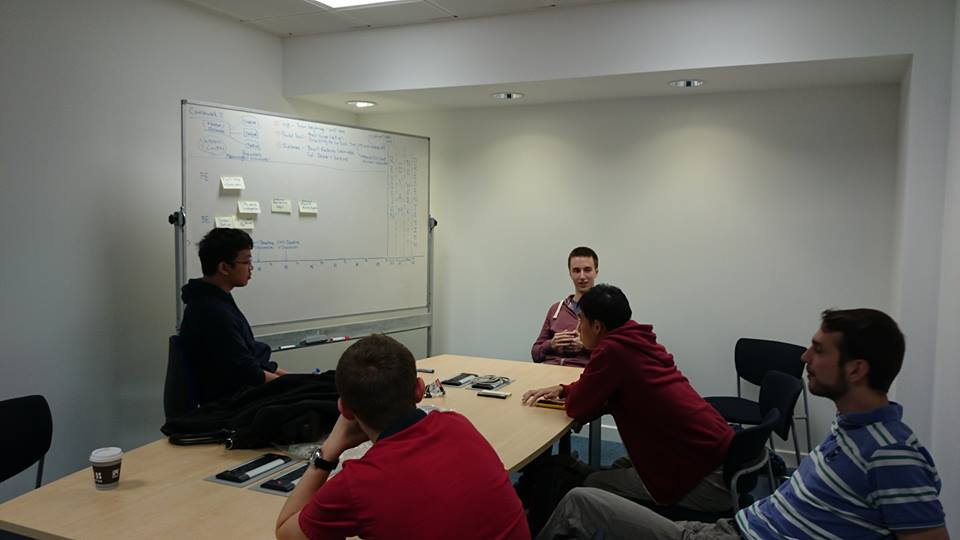
\includegraphics[width = 0.99\textwidth]{./planning/scrum.jpg}
   
  \caption{Half-weekly ``scrum'' (development team meeting).}
  \label{fig:scrum}
\end{figure}

\subsubsection{Technical Practices}

We also integrate a few technical practices inspired by Extreme Programming:
\begin{itemize}
  \item \textbf{Pair Programming}: as mentioned in section \ref{sec:projman_group}, we sorted
        ourselves into three pairs, focusing on frontend (FE), backend (BE) and database (DB) work.
        Such a practice allows continuous development on all divisions without
        being affected by instances in which a member is required to temporarily shift his or her
        focus from the project to other coursework/tests.
  \item \textbf{Test-driven Development}: during development, we will constantly be writing small tests to make sure individual features are working as expected before we move on to the next feature.

\end{itemize} 

\subsubsection{Project Tracking}

Finally, to keep track on the group's progress, we use an electronic task
board on Trello (see figure \ref{fig:trello}). Here we can assign ourselves (and others) specific tasks and a general due date. Trello allows us to see what the other members of the group are doing and when a feature is expected to be completed. We can also easily add photos and checklists to see how the project is forming. We decided to use Trello as a physical story-board is not feasible. As well as Trello, we will constantly be communicating personally in labs, online via messaging services, and regular stand-ups in a meeting room. This development process is a feature of the Kanban methodology.

We chose to incorporate this into our way of working, as one of the team members, Andrew, had worked with Kanban previously, and found it very useful to visualise the work being done on a project.

\begin{figure}[ht]
  \centering
%    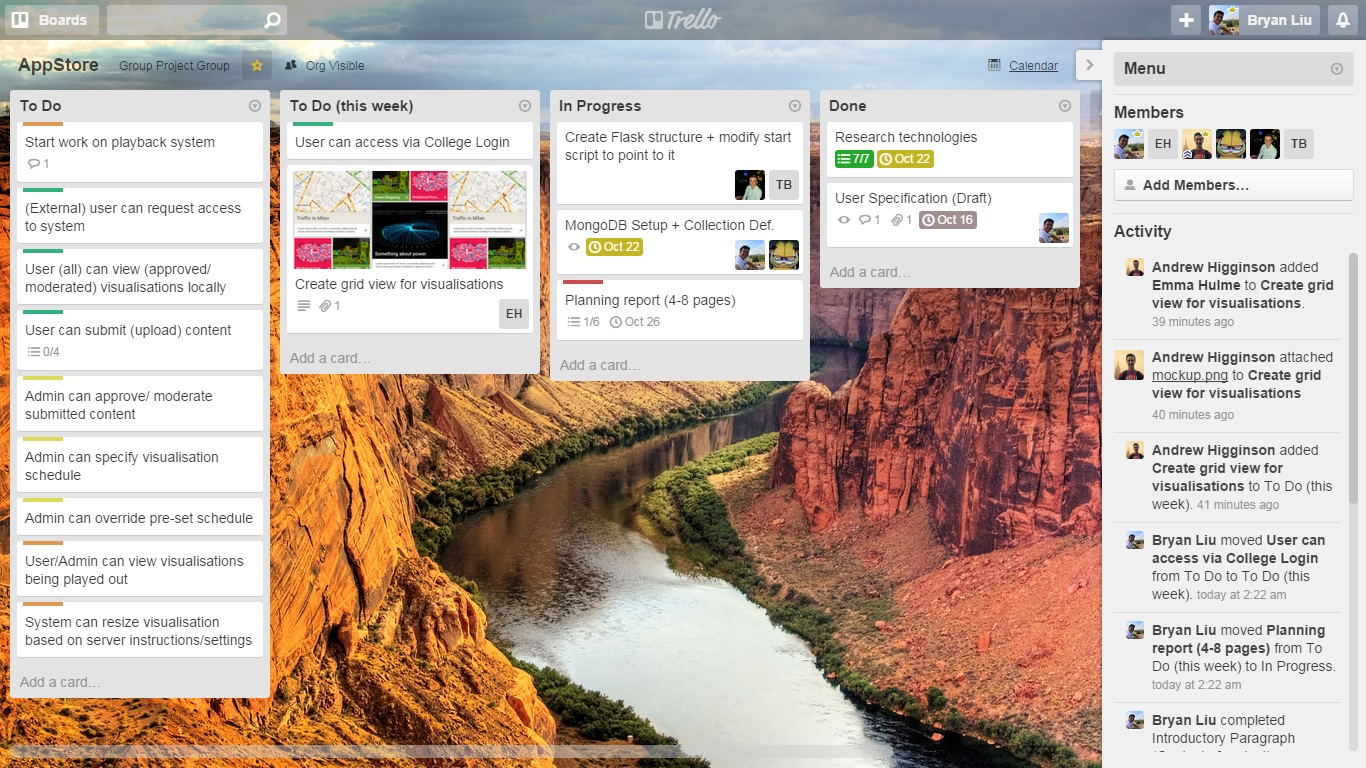
\includegraphics[width = 0.99\textwidth]{./planning/trello.jpg}
   
  \caption{Using Trello to keep track of progress.}
  \label{fig:trello}
\end{figure}

\subsection{Development Tools}

\begin{figure}[ht]
  \centering
%    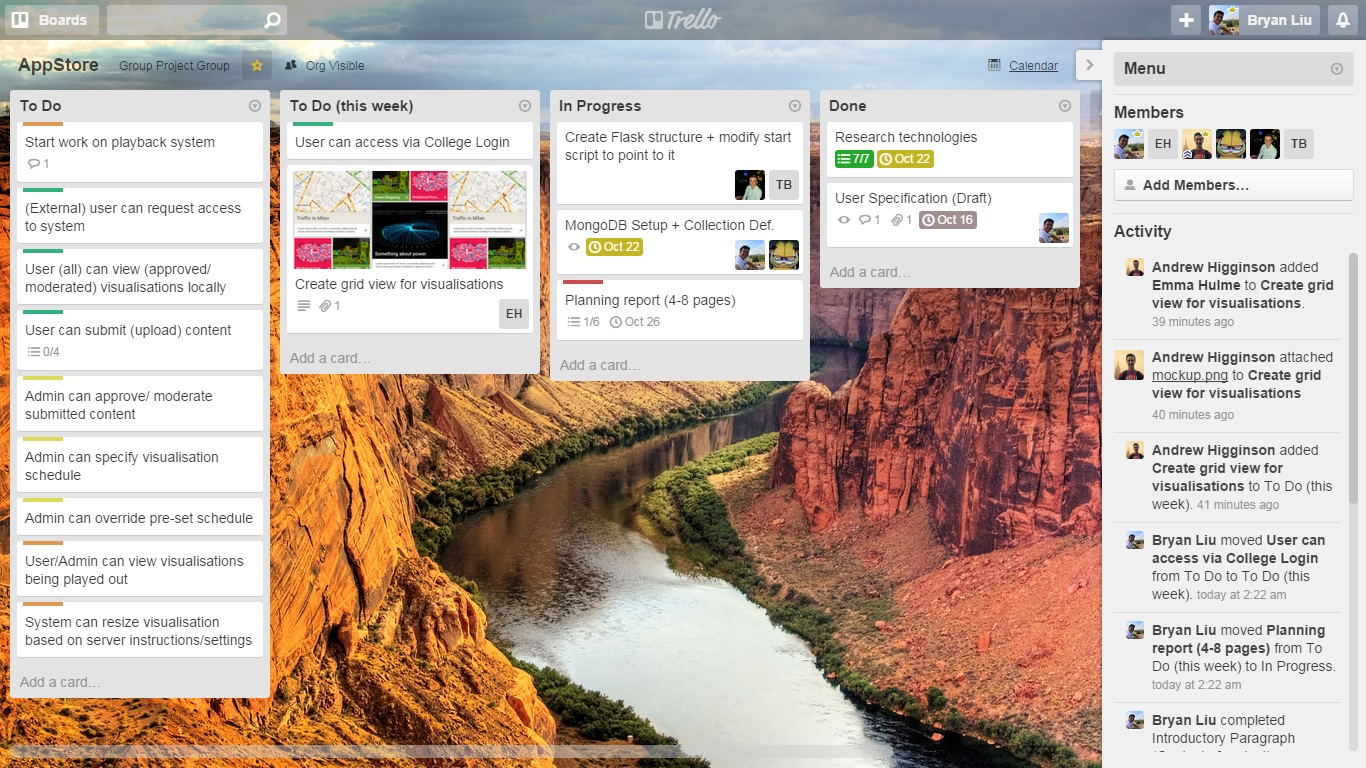
\includegraphics[width = 0.99\textwidth]{./planning/trello.jpg}
   
  \caption{Development methods and tools utilised in project.}
  \label{fig:trello}
\end{figure}
During the inital phases of our project, we decided on which tools/technologies to use based on our personal preference. For the backend, we decided to use Python with Flask. Members of our team had previously used Ruby on Rails and Python with Django, so we decided to use Flask for interest purposes. To make sure Flask was suitable, the backend team spent time researching additional modules that would allow us to implement future features. We found that Flask met this criterion.

As Bryan and Jackie were more interested in the database side, they chose to use MongoDB as a NoSQL solution. Again, this was based on interest. Bryan used time at the beginning of the project to check that Flask was compatible with MongoDB. 

For the frontend, given the amount of similar web application projects Andrew and Emma had worked on, they decided to explore using AngularJS, as a different way of implementing frontend logic. They have since decided to use it, as it allows interfaces to be programmed declaratively, making it much easier to 'see the behaviour' of the UI from code.

After a lecture on deployment techniques, the group decided to use Docker. In a group project last year, the backend team had to wait if the frontend was broken to see if particular feature was working. Using Docker and extra virtual machines (created on the department's cloudstack), we can have a separate machine for each feature while it is in development, and have multiple copies of the web server running. Docker allows us to quickly set up the virtual machines via a script, installing any dependencies we need automatically. Although it may be a steep learning curve at the start of our project, Docker will save us a lot of time later. 

We have yet to concretely decide on the best solution for our playout system, as this is relatively independent of the technologies used for the web service. Andrew briefly explored possible options and there is a high probability we will use the Qt toolkit, as it is a widely used, cross-platform option, however this will be decided in one of our weekly meetings nearer the end of our project.

As usual, all of our code (including the Docker scripts) will be stored in a group git repository. As a group, we have decided to use branches with a short lifetime. Each minor feature will be implemented on it's own branch, with the master (or trunk) branch used for merging in features only. Merging will take place after the feature is tested on its own branch and VM. 

To deploy the webserver, David has provided us with a Linux VM with root access. Setting up this VM will simply be a case of running our existing scripts with Docker. The playout software will be run on a dedicated computer hooked up to the four projectors, which will be provided by David. 


\subsubsection{Version Control}

\subsubsection{Unified Development Envorinment}

\subsubsection{Test-driven Development}

\subsubsection{Continuous Integration \& Build Promotion}


\newpage
\section{Design and Implementation}

\newpage
\section{Evaluation}

\subsection{Stakeholder Relationships}

\subsubsection{Stakeholders}

The main stakeholder in our project is our supervisor, David. The core of our project is the scheduling component, which he will operate as an administrator, so his opinion of the overall design of the project is critical.

Our second class of stakeholders are those who browse the visualisation catalogue and submit visualisations and advertisements. Their stake is relatively large as without their full engagement and satisfaction, the variety of content being shown will remain small. 

Our last group of stakeholders are those who see the visualisations being played out. While this set of users are still important, their stake is relatively small, in that all they want to see is the content being played out successfully.

\subsubsection{Customer relationship}

Where customer relationships are concerned, we see our most important stakeholder, our supervisor, David, as somewhere between an internal and external customer, whom we hold weekly meetings and exchange emails frequently with but not contact in person daily. During weekly meetings, we explain the features that are in progress/to be done over the next week, so that David is always kept in the loop (Figure \ref{fig:meetingboard}).

We tended to keep discussions fairly high-level, and only discussed implementation details/technologies when asked to do so, or when we felt that it was important to the discussion. We did this to mimic the scenario of David being our client, but also to ensure that discussions were not biased towards any kind of implementation, allowing us to fit our implementation around the best ideas, and not the other way around.

\begin{figure}[H]
  \begin{minipage}{0.49\textwidth}
    %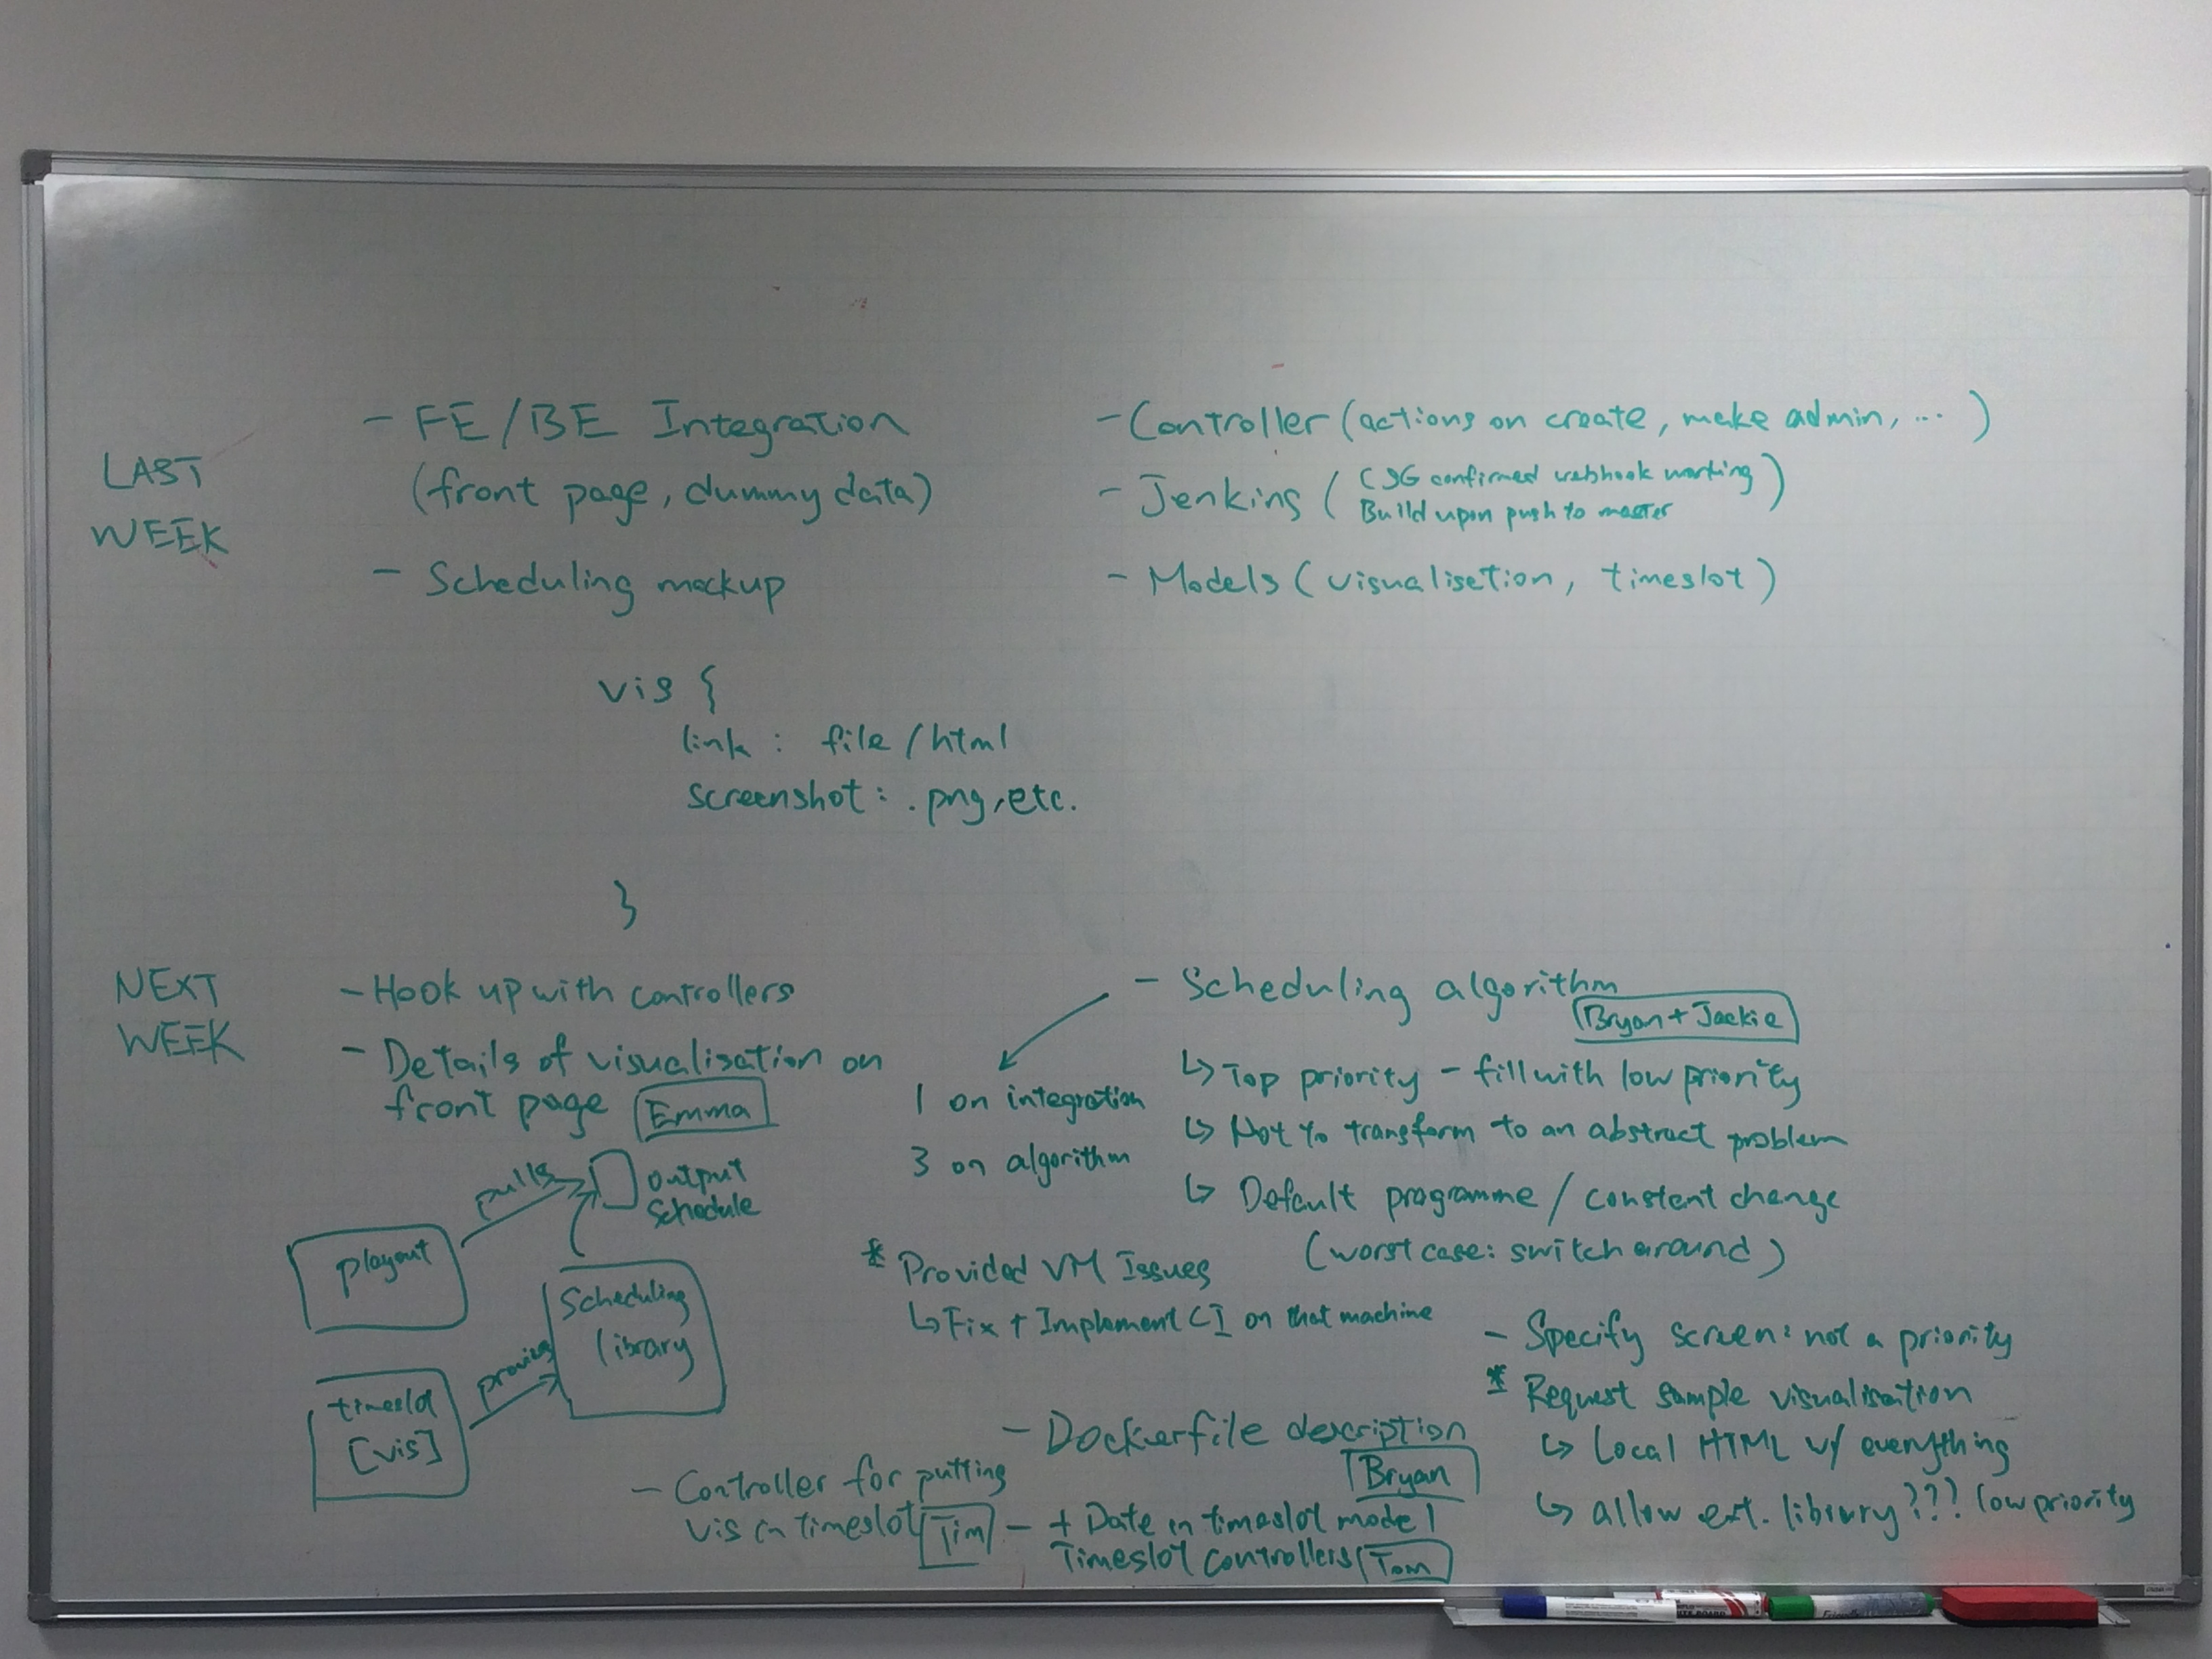
\includegraphics[width = \textwidth, trim = 0 0.4cm 0 1.6cm, clip]{./evaluation/meeting-board2.jpg}
  \end{minipage}
  \begin{minipage}{0.49\textwidth}
    %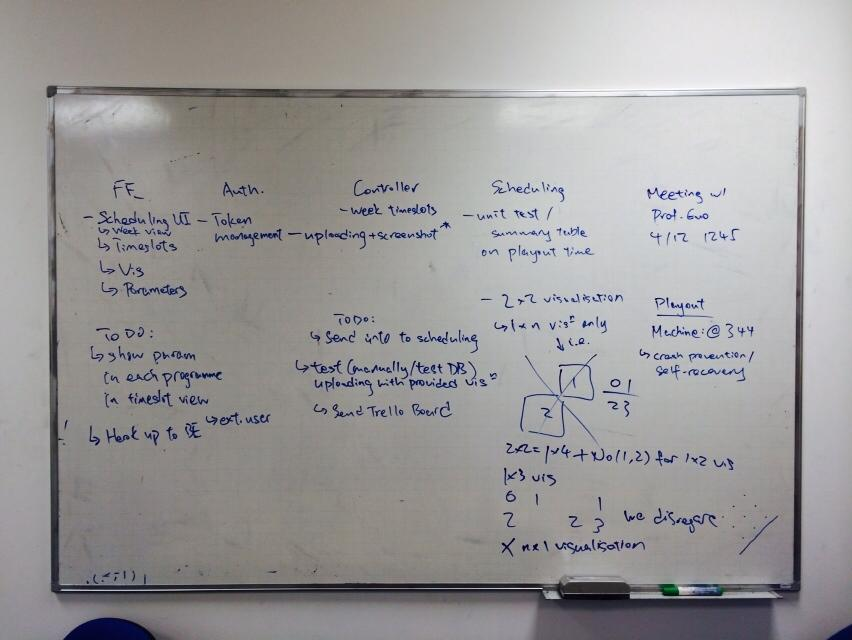
\includegraphics[width = \textwidth, trim = 1.2cm 1.5cm 1.2cm 2.5cm, clip]{./evaluation/meeting-board.jpg}
  \end{minipage}
  \caption{Meeting notes with group progress and feedback from David (our supervisor) after sprint cycles 2 (left) and 4 (right).}
  \label{fig:meetingboard}
\end{figure}

Furthermore, with the aid of Jenkins, we are able to give the address of our ``release VM'' to David, where he can see the latest working version of the project. From this, David can constantly evaluate and provide feedback on our project features through all stages of development.

\subsubsection{Feedback handling}

Upon receiving feedback from our stakeholders, mainly from our supervisor, we handled them depending on their nature:

\begin{itemize}

  \item Change in minor details of a feature/design: \\
        Usually happening in the prototype stage, they include changing font size/colour and displaying some extra information on a screen. As these changes take only a few hours at most to implement, we took the majority of such suggestions and fitted these XS-items in the next iteration.

  \item Introduction of new, peripheral features: \\
        These include features that are related but not essential for our three main components (submission, moderation/scheduling and playout): Multiple default playout lists, playing videos with linked themes consecutively, buttons to copy and paste previous timeslots, etc. \\
        However, due to time limitations, we chose to integrate only one or two small-sized features into our planned implementation. The rest of the suggested features were put into an ``extra feature" list, which we only considered implementing after basic versions of the main components are completed. This ensures that we can produce a minimal product at the very least before our planned deadline.

  \item Major changes in feature implementation: \\
        As a result of differing assumptions, the feedback necessitates the changing of what we have already implemented. For instance, we were required to change the priority rules in our scheduling algorithm. When this happens, we spend a significant portion of the weekly meeting to clarify the assumptions that our supervisor has made, and try to combine them with our own assumptions and implementations. This feedback has sometimes resulted in some or all of our code being scrapped, but it generates a product which is more useful to our stakeholders.

\end{itemize}

In all cases, we have communicated with the personnel that provided the
feedback with justification on our decisions. For example, we told
our supervisor that we are happy to accede to his request of adding a button which copies previous timeslots as we rate it as a S-sized task which can fit into the planned iteration, but his request for linked videos to be scheduled to be screened consecutively would delay our plans, and thus should be considered only after the entire system is implemented minimally.

\subsection{Product Requirement, Value \& Impact}

In the first week of embarking on our project, we met with our supervisor to highlight the initial components required. At first, these were general
requirements including:

\begin{itemize}

  \item Stakeholder requirements resembling user stories (e.g. a user is allowed to submit scientific visualisations and/or advertisements, as well as to state his/her preference(s) on playout).

  \item System/Interface requirements - what users expect it to be able to do based on the user stories above (e.g. The scheduling system should schedule items to play out in rotation, so that passers-by will not be bored by the ``fixed" playout sessions).

\end{itemize}

\begin{figure}[H]
  \centering
    %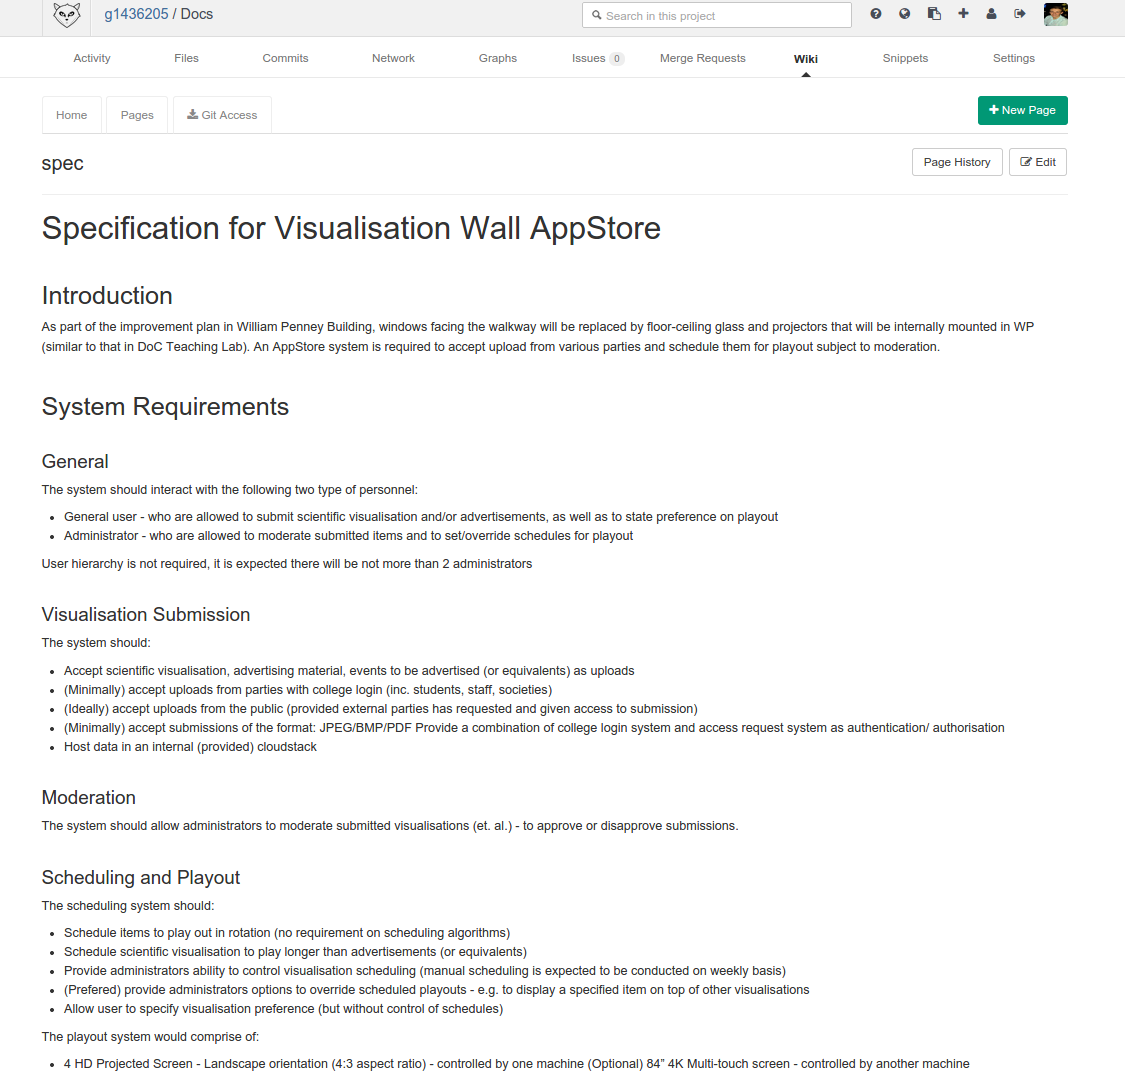
\includegraphics[width = 0.9\textwidth, trim = 0 15cm 0 5cm, clip]{./evaluation/specs.png}
  \caption{Initial specifications (partial) on shared repository.}
  \label{fig:specs}
\end{figure}

In the following weeks, we then clarified and expanded on these requirements as a group. This allowed us to discuss the implementation and technical details of specific features.

\subsubsection{Value Proposition}

We also further clarified our understanding of stakeholders and how our system creates value for them via multiple value proposition canvasses. Figure \ref{fig:valpropcanvas} shows the canvas for the Imperial Data Science Institute, which our supervisor is associated with. It includes a customer profile with a list of jobs, gains and pains, and corresponding products/services, gain creators and pain relievers (value map). Some of the gains/pains of the institute, along with their creators/relievers are as follows:

\begin{itemize}

  \item Gain: Makes the walkway more interesting (by showing visualisations to passers-by)

  \item Pain: Requires a large number of visualisations (relieved by inviting users to submit visualisations)

  \item Gain: Creates income opportunities (by showing adverts)

  \item Pain: Attracts inappropriate submissions from users (relieved through admin moderation)

\end{itemize}

The canvasses enable us to disregard features that deliver low or no value, and make more reasonable assumptions about our stakeholders. We believe that the latter has resulted in fewer problems for us when we began our product validation, detailed in Section \ref{sec:validation}.

\begin{figure}[H]
   \begin{center}
      %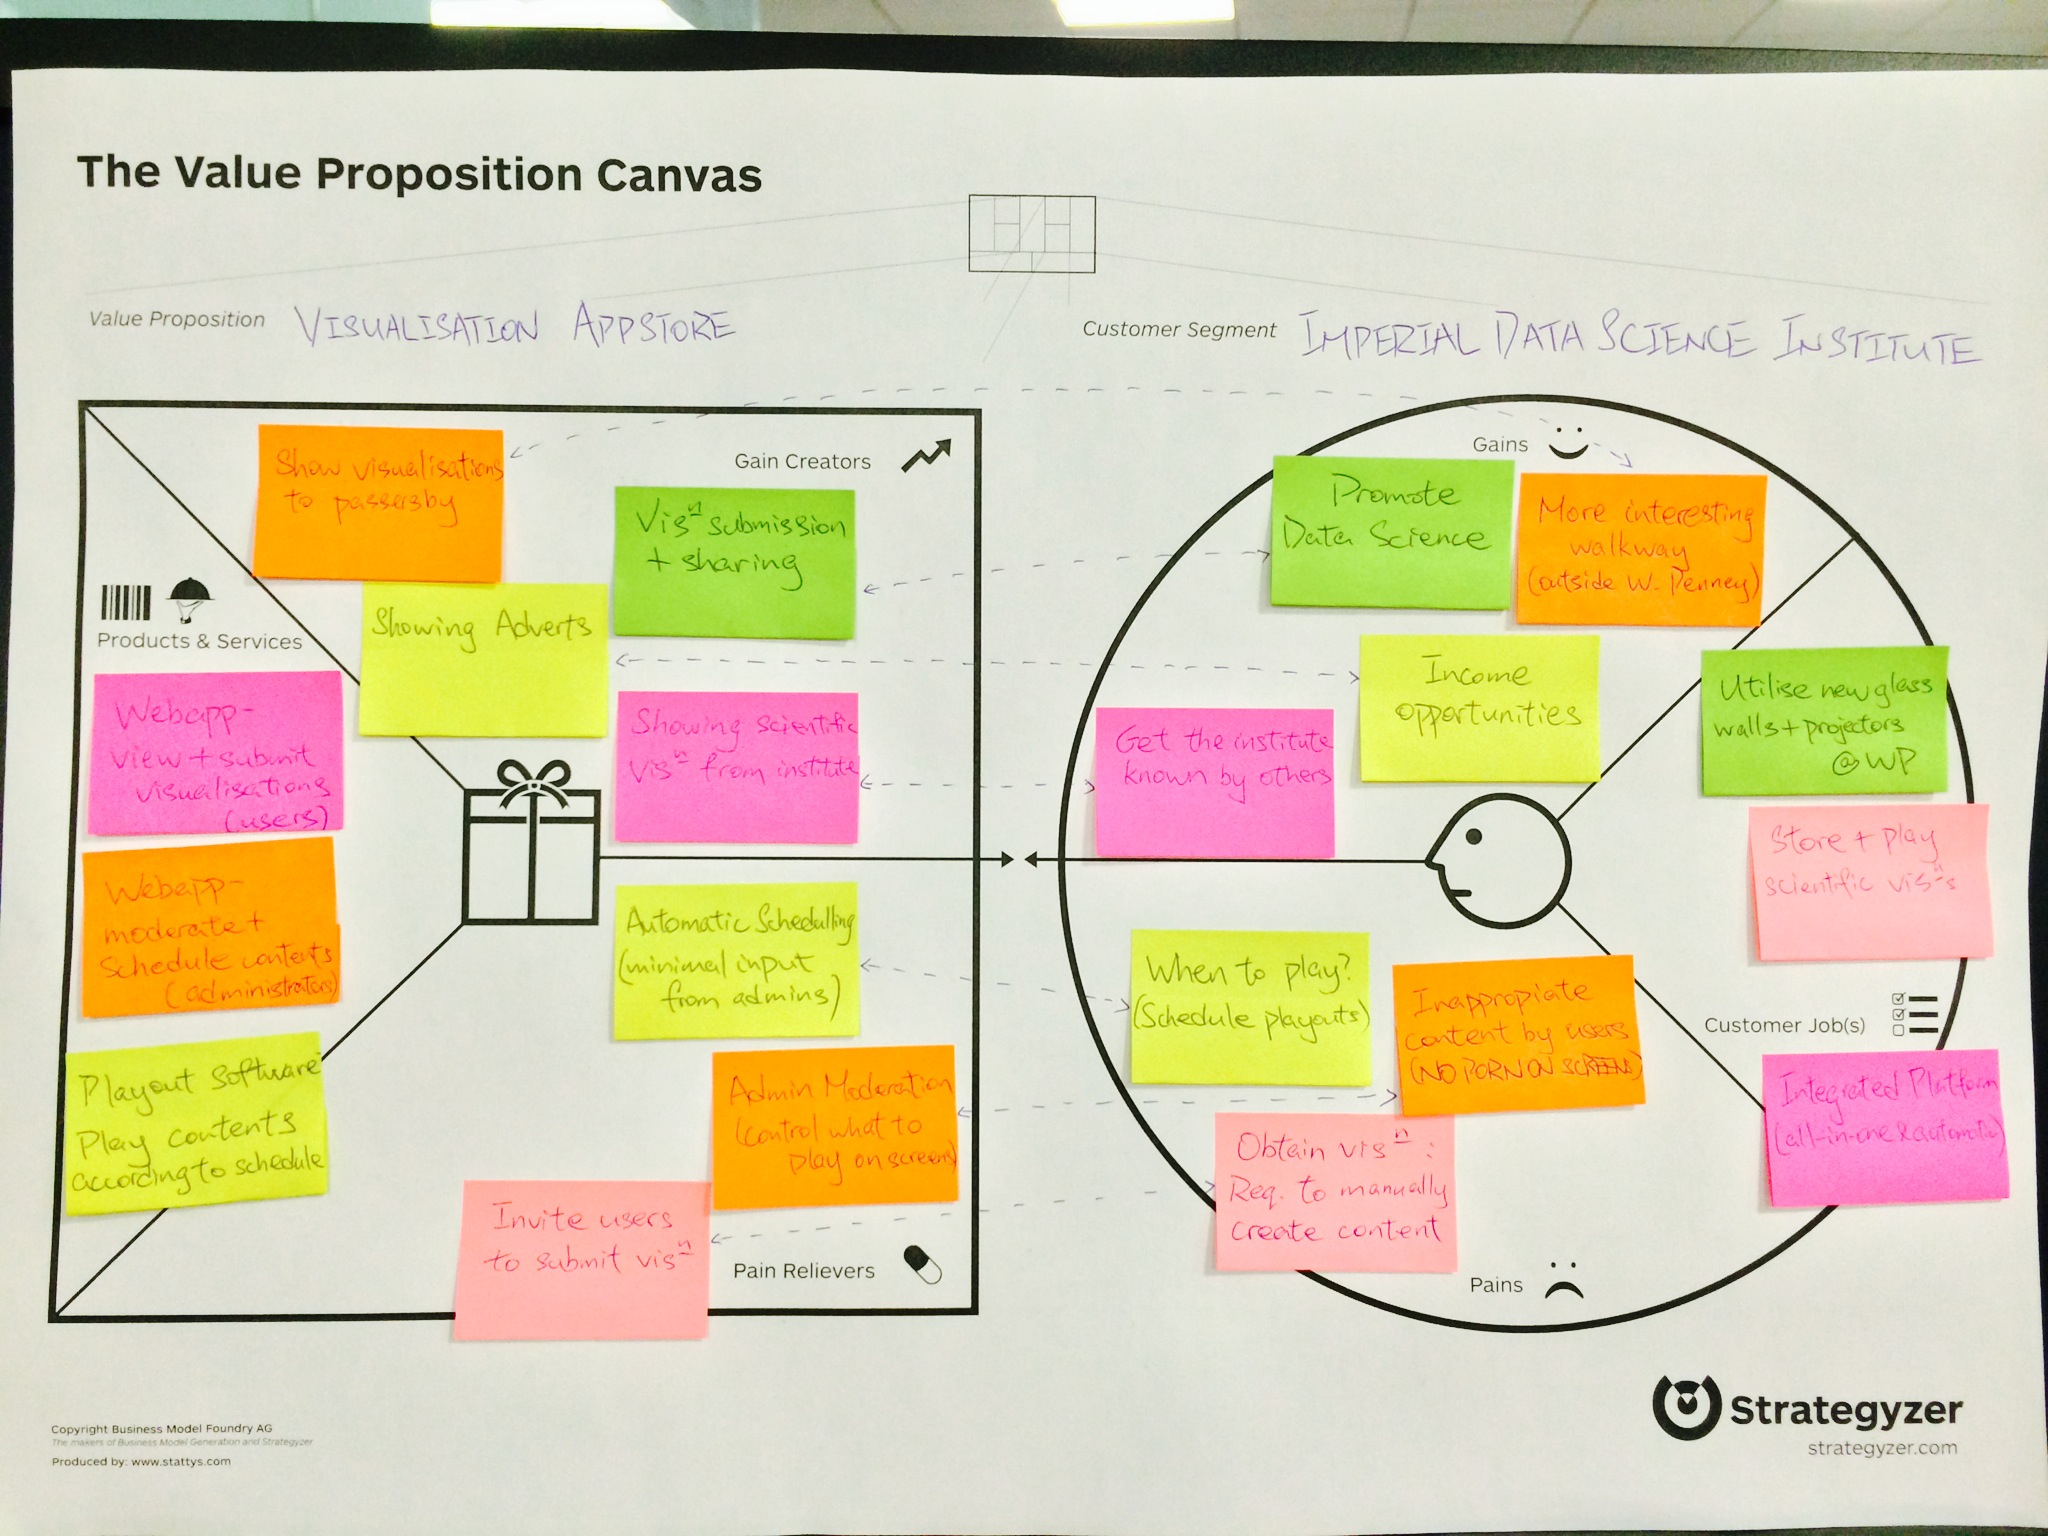
\includegraphics[width = 0.9\textwidth, trim = 1cm 6.5cm 1cm 4.5cm, clip]{./evaluation/value_prop_canvas.jpg}
   \end{center}
   \caption{Value proposition canvas for our client (Imperial Data Science Institute).}
   \label{fig:valpropcanvas}
\end{figure}

\subsection{Task Management}
%TODO: if required to expand

During development, we constantly looked at the requirements from all of our stakeholders, which we stored in a shared document. In our weekly scrums, we presented the work that we have done to one another and discussed whether the project is on the right track.

We prioritised tasks on our Trello board using different columns. In addition, we constantly communicated both face-to-face and online, to make sure that group members are implementing assigned tasks at the right times. We also used the Trello board actively to update the rest of the group when tasks have been completed, hence saving us the trouble of constantly asking the rest of the group or looking at code to find out if a feature has already been implemented. When appropriate, group members working on the backend used an internal wiki on Gitlab to provide information about routing, controller actions, and parameters. 

\begin{figure}[H]
  \begin{minipage}{0.49\textwidth}
    %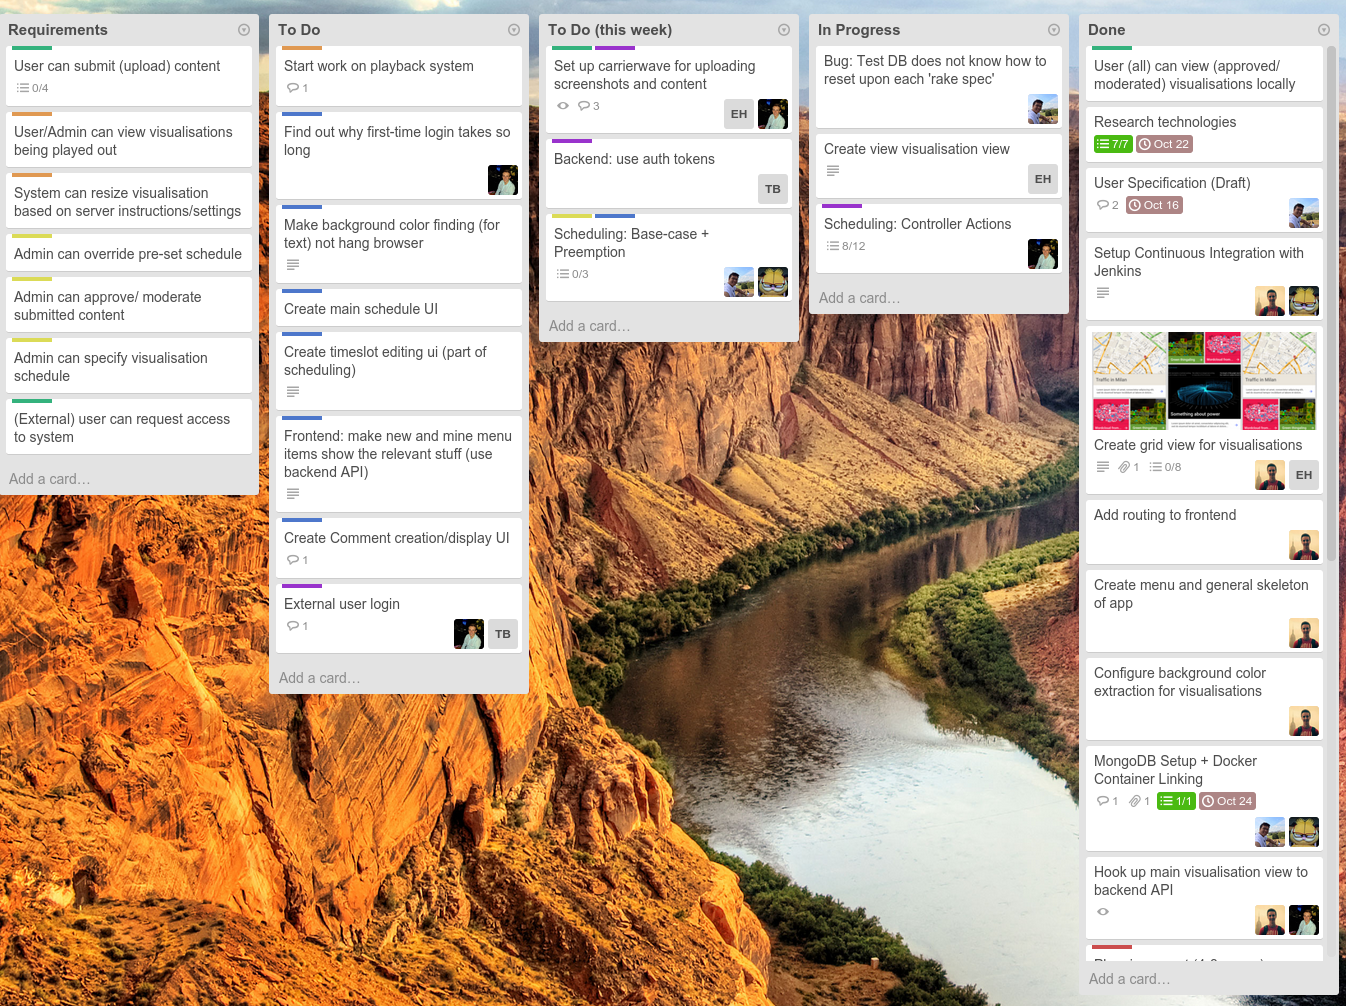
\includegraphics[width = \textwidth]{./evaluation/trello-columns.png}
  \end{minipage}
  \begin{minipage}{0.49\textwidth}
    %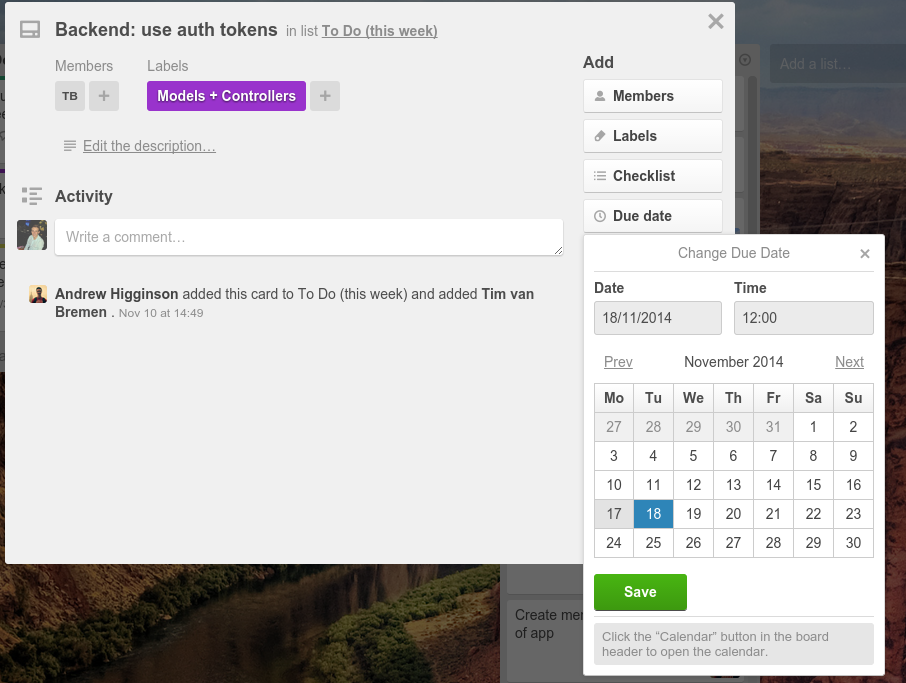
\includegraphics[width = \textwidth]{./evaluation/trello-due-date.png}
  \end{minipage}
  \caption{Priority columns on our Trello board (left), and \\ setting a due date for a particular task (right).}
  \label{fig:trello}
\end{figure}

\subsubsection{Story Splitting}

While some of our project requirements can be completed within a few hours, other features are unlikely to be completed within one iteration. In such cases, we split the features into multiple units and implement them in different iterations based on their priority.

An example can be found in the following user story:
\begin{center}
``\textit{As a user, I want to access the platform via a set of credentials so that I can upload visualisations (user)/perform moderation and scheduling (administrator).}'' \\
\end{center}

We considered this task to be technically challenging. Hence, we split it into the following subtasks:

\begin{itemize}

  \item As an internal user (student/staff at Imperial), I want to access the platform via my college login so that I can upload/moderate and schedule visualisations without the need for an extra set of credentials.

  \item As an external user, I want to access the platform via some kind of access request system, so that I can share my visualisations too.

\end{itemize}

In addition to being reduced in size, splitting the story has also helped us further understand the needs of different groups of users. As such, we decided to implement the former requirement first, as some of our team members have had experience on working with the college login system, hence allowing the requirement to be fulfilled in a shorter time. The latter requirement was then scheduled to be carried out in parallel with the mentioned features.

\subsubsection{Spikes - Experiments with new technologies}

Throughout development, we also devoted a small proportion of time to experiment on technologies involved in later iterations. This allows us to better understand the potential complications that we will face and react accordingly.

While we planned to implement the playout system only in iterations 5 and 6 (the last two iterations), investigation on relevant technologies, including Qt and its adapters, were made from iteration 2. Preliminary research allowed us to confirm that 2 weeks would be a reasonable estimate in system implementation. Furthermore, we believe that the investigation would result in a more gentle learning curve, and reduces the risk for development grinding to a halt as team members will at least have some basic knowledge on Qt, and some code segments will be produced.

However, not all spikes bring good news - investigation on Kerberos login libraries has revealed that the adapter for Flask (with Python) is actually broken, forcing us to scrap the entire implementation. Nonetheless, the spike allowed us to switch our choice of development language early and avoid incurring high costs further into development.

\subsection{Building the right thing - Assumption Validation} \label{sec:validation}

Given the tight deadlines for the entire project, we agreed to collect
user feedback as soon as the project commenced. This ensures that we are building the right product for our stakeholders.

\subsubsection{UI mockups/ prototypes} \label{sec:uimockup}

Before implementing a particular part of our project, we begin with creating mockups (Figure \ref{fig:mockup}). These can be produced in a relatively short time, and allows us to quickly think through the design of our project, without being tied down to any implementation details. After completion, we show the mockups to the main stakeholder in the project i.e. our supervisor, who gives us feedback. For example, he mentioned that it will be a good idea to show the priorities associated with each visualisation in the timeslot views, even if the visualisation is not selected after viewing the mockups.

Once we have settled on a general design, we complete the main implementation of the UI within that week's sprint cycle, but only up to the point where we can see how it will be used. As it is not interacting with the backend at this point, small changes are easily implemented, with the following week's sprint cycle involving ``hooking'' up this UI prototype with our backend.

We also made sure that this prototype is seeded with some dummy/representative data in some way, so that it is clear how each part of the project will operate in practice.

\begin{figure}[H]
   \begin{center}
     % 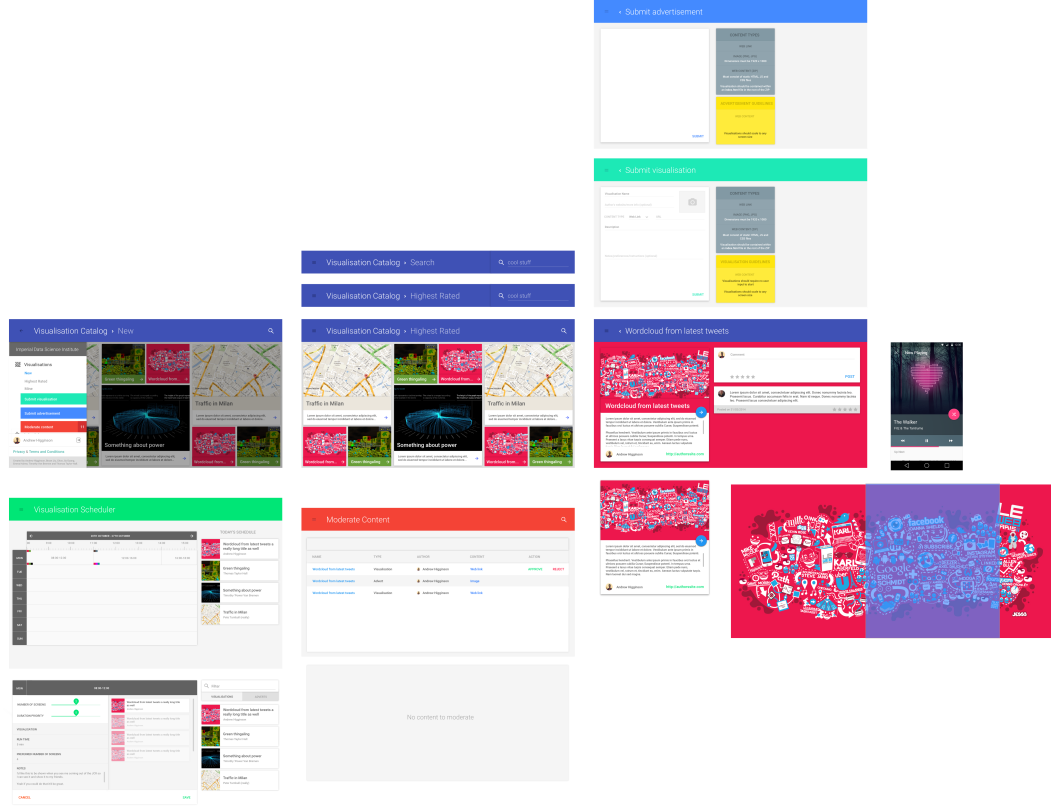
\includegraphics[width = 0.9\textwidth, trim = 0 0 0 0cm, clip]{./evaluation/mockup.png}
   \end{center}
   \caption{Mockups on User Interface}
   \label{fig:mockup}
\end{figure}

\subsubsection{Requirements on intangible ideas}

Compared to UIs which users can see and feel, we believed that uncovering the client's assumption on playout scheduling via mockups or prototypes will not be feasible as the scheduling algorithm is mainly rule-based. Instead, we delivered our ideas to our supervisore with whiteboard illustrations, and recorded his feedback.

Throughout these discussions, we uncovered several assumptions made by our supervisor, one of which is expecting the scheduling algorithm to ensure that playout time is directly proportional to metric set by administrators. In response, we have created additional unit tests to incorporate such requirements in our scheduling algorithm.

\begin{figure}[H]
  \begin{minipage}{0.46\textwidth}
     % 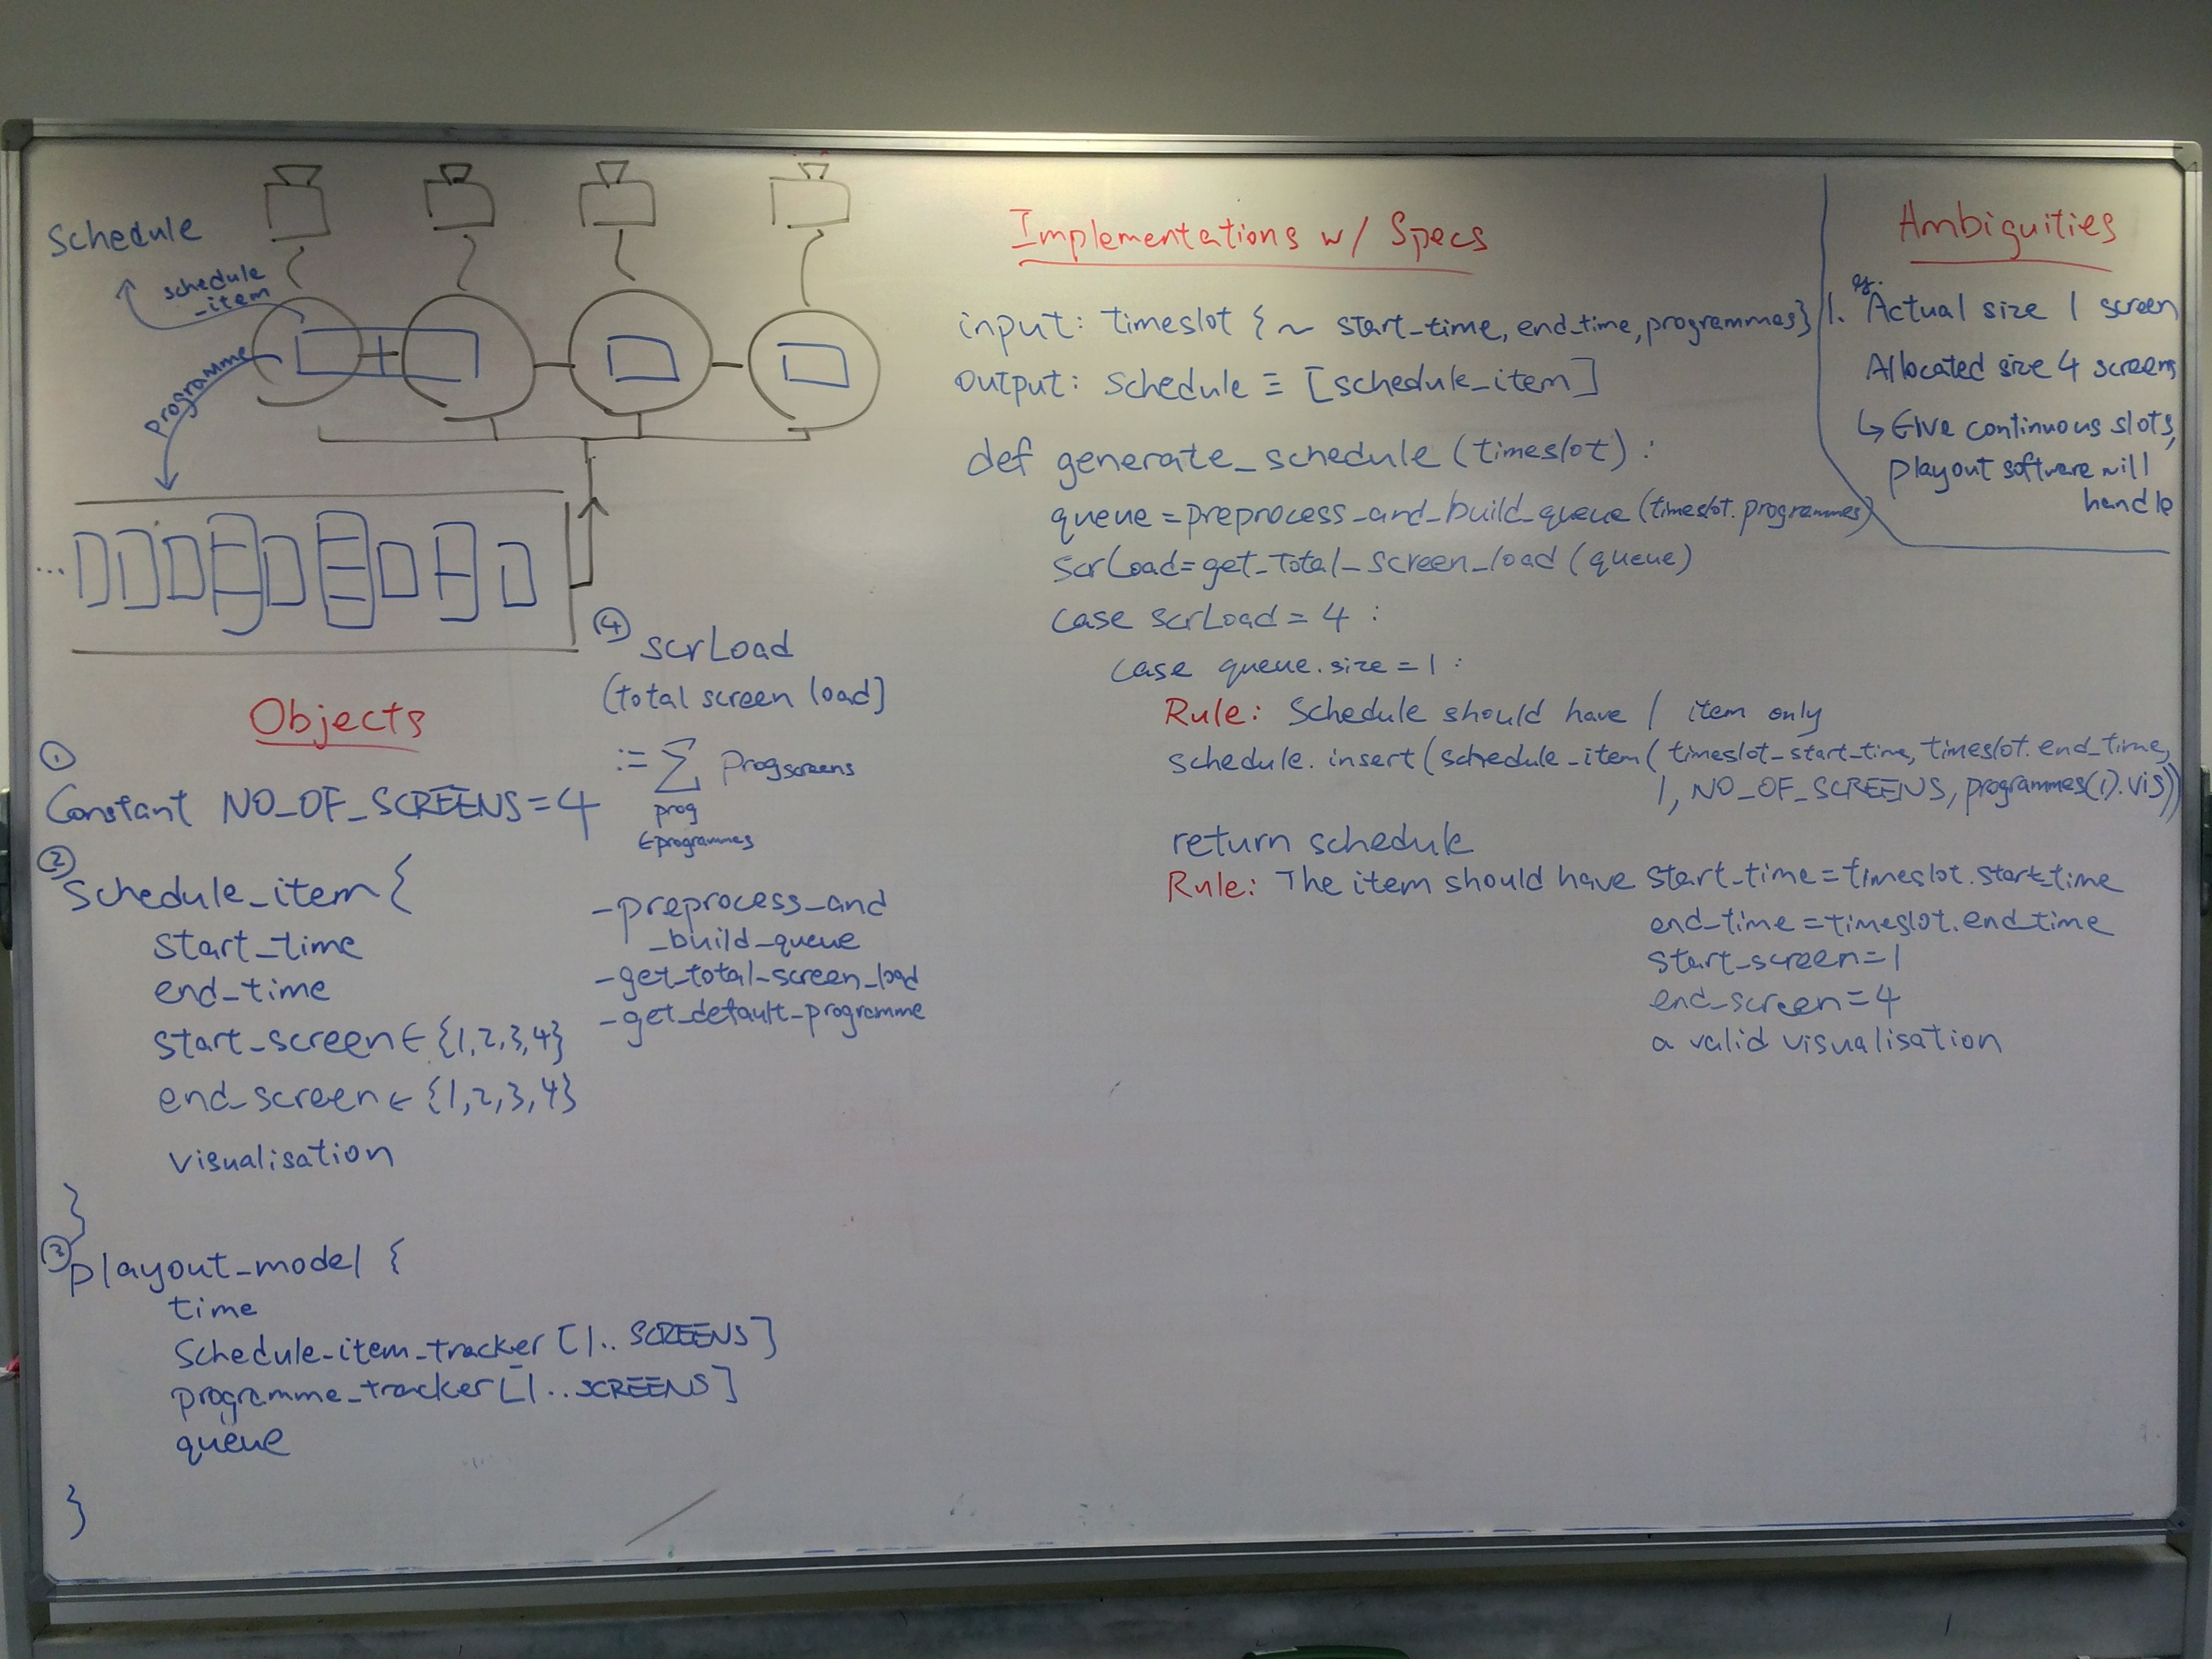
\includegraphics[width = 0.99\textwidth, trim = 0 1cm 0 1.5cm, clip]{./evaluation/scheduling_whiteboard.jpg}
  \end{minipage}
  \begin{minipage}{0.53\textwidth}
     % 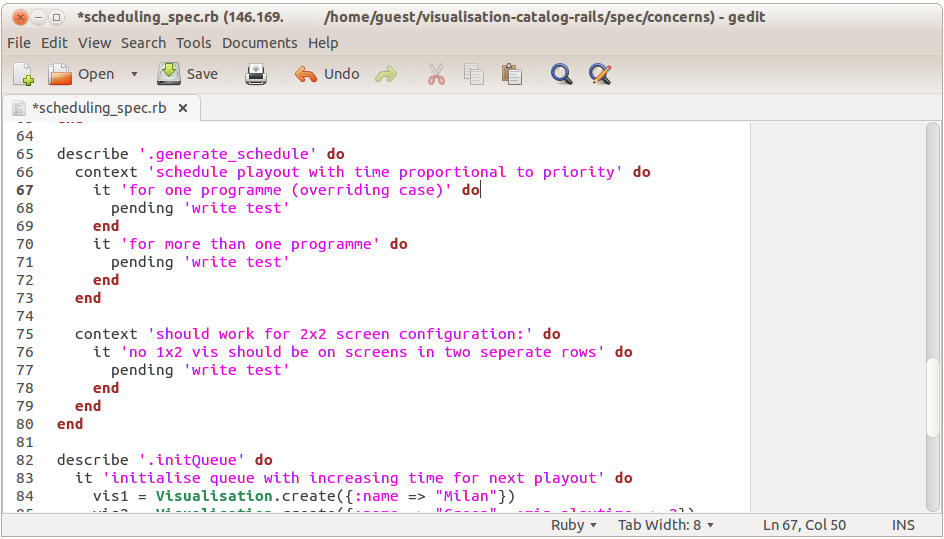
\includegraphics[width = 0.99\textwidth]{./evaluation/scheduling_spec.png}
  \end{minipage}
  \caption{Capturing scheduling requirements on whiteboard (left), \\ and subsequently via RSpec unit tests (right)}
 
\end{figure}

\subsubsection{User testing}

We also conducted implicit user tests during demonstrations of new features, where we asked our supervisor to complete certain tasks with minimal instructions and guidance (e.g. to navigate to the visualisation scheduling page and schedule some visualisations for playout).

Such testing allowed us to learn what is evident to us but obscure to our users. For example, in one of our demonstrations, we observed that our supervisor made multiple pauses when asked to navigate to the moderation and scheduling pages. This indicated that the icon showing the user menu may not be obvious enough to users, and the description for menu items may not be clear enough. Based on such observations, we changed the size of the ``show menu'' button, and also explored the effect of various font colours on the user menu.

We are planning to extend this user testing to include more potential users, especially those that are ranked second in our list of stakeholders, such as staff and students who may use the platform to submit and 
view visualisations.

\subsection{Evaluation}

Even as we are able to evaluate the correctness of our project by unit and system tests after a feature is implemented via RSpec, we still require some other means to test the quality of our features, as well as our group's progress.

\subsubsection{Validated learning \& Pivoting}

As mentioned in Section \ref{sec:validation}, obtaining feedback via mockups, prototypes with representative data and user testing allowed us to 'pivot' many times with minimal reimplementation overhead. It also allows us to identify problems or learn more about the issues that we are trying to solve, before we write large volumes of code which may end up to be not useful. Moreover, this lean approach \textbf{encourages us} to pivot more often, as there is no reason not to do so.

\subsubsection{Project progress}
	
Quantitatively, we evaluated our project by tracking how fast we were ticking off our initial requirements. Using our Trello board and version control system, we can easily see by whom and at what time each feature has been implemented. By combining these with our estimates of the size of each task, we are able to analyse the group's performance via a Cumulative Flow Diagram (Figure \ref{fig:cumuflow}).

\begin{figure}[H]
  %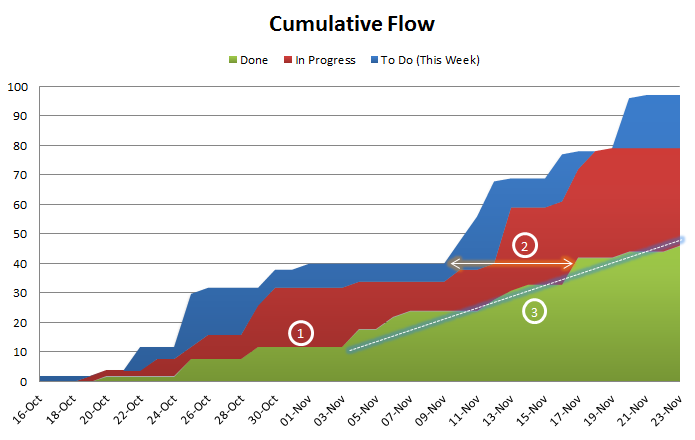
\includegraphics[width = 0.99\textwidth]{./evaluation/cumu_flow.png}
  \caption{Cumulative flow diagram for our team based on tasks' status}
  \label{fig:cumuflow}
\end{figure}

The diagram tracks the tasks on the columns ``To Do (This week)", ``In Progress" and ``Done", where each task carries a story point based on their size estimate. From the diagram, we can make the following observations:

\begin{enumerate}

  \item In the last week of October, the group did not make much headway for in-progress and to-do tasks. This observation is attributed to problems in setting up Jenkins, which caused a bottleneck in the entire development process.

  \item The lead time (time required between starting and completing a task) is usually around 2 weeks. Given the way we work on a new feature (2 cycles per feature - detailed in Section \ref{sec:uimockup}), we believe that we are making healthy progress in getting individual components of our project done.

  \item Within the first 3 weeks in November, the team has completed tasks worth 35-40 story points. Given that the minimal system is estimated to be worth $\approx$90 story points, we believe that we will be able to meet our deadline in the second week of December with a similar effort.

\end{enumerate}


\newpage
\section{Conclusion}

\subsection{Future Extensions}


% -- Appendix
\newpage
\appendix

% -- Initial Spec
\section{(Initial) Specification for Visualisation Wall AppStore}

\textbf{\Large Introduction}

As part of the improvement plan in William Penney Building, windows facing the walkway will be replaced by floor-ceiling glass and projectors that will be internally mounted in WP (similar to that in DoC Teaching Lab). An AppStore system is required to accept upload from various parties and schedule them for playout, subject to moderation.\\

\textbf{\Large System Requirements} \vspace{5pt}

\textbf{\large General}

The system should interact with the following two type of personnel:

\begin{itemize}
  \item General user - who are allowed to submit scientific visualisation and/or advertisements, as well as to state preference on playout.
  \item Administrator - who are allowed to moderate submitted items and to set/override schedules for playout.
\end{itemize}

User hierarchy is not required, it is expected there will be not more than 2 administrators.\\

\textbf{\large Visualisation Submission}

The system should:

\begin{itemize}
\item Accept scientific visualisation, advertising material, events to be advertised (or equivalents) as uploads
\item (Minimally) accept uploads from parties with college login (inc. students, staff, societies)
\item (Ideally) accept uploads from the public (provided external parties has requested and given access to submission)
\item (Minimally) accept submissions of the format: JPEG/BMP/PDF Provide a combination of college login system and access request system as authentication/ authorisation
\item Host data in an internal (provided) cloudstack\\
\end{itemize}

\textbf{\large Moderation}

The system should allow administrators to moderate submitted visualisations (et. al.) - to approve or disapprove submissions.\\

\textbf{\large Scheduling and Playout}

The scheduling system should:

\begin{itemize}
\item Schedule items to play out in rotation (no requirement on scheduling algorithms)
\item Schedule scientific visualisation to play longer than advertisements (or equivalents)
\item Provide administrators ability to control visualisation scheduling (manual scheduling is expected to be conducted on weekly basis)
\item (Prefered) provide administrators options to override scheduled playouts - e.g. to display a specified item on top of other visualisations
\item Allow user to specify visualisation preference (but without control of schedules)
\end{itemize}

The playout system would comprise of:

\begin{itemize}
\item 4 HD Projected Screen - Landscape orientation (4:3 aspect ratio) - controlled by one machine 
\item (Optional) 84” 4K Multi-touch screen - controlled by another machine
\end{itemize}

The playout system would:

\begin{itemize}
\item Size visualisation (or equivalents) automatically (e.g. scale fluidly) (Highly possibly) be web-based and playout via browsers
\item Be run from 8am - 8pm (but should be built to run arbitrary hours)
\item Be scalable in projecting on screens (e.g. 4x1 or 2x2 configuration)\\
\end{itemize}

\textbf{\large Security}

The system should be secure from external interference, especially for playouts.\\

\textbf{\large Miscellaneous}

\begin{itemize}
\item The system should provide an RESTful API for third-party upload/ playout.
Development standards/requirements are welcomed for visualisation, but should be kept minimal for general web pages be shown
\item The system should be branded under Imperial’s Data Science Institute\\
\end{itemize}


\textbf{\Large Available Technologies/ Resources} \vspace{5pt}

\textbf{\large 4x HD Projection Screen}

Screens are controlled by a single, custom machine with graphics card via HDMI cables. It is believed that Windows provide better driver support yet it is fine to run on Linux as long as Chrome is able to be run.\\

\textbf{\large 84” 4K Multi-touch Screen}

The multi-touch screen is run by a dedicated machine in Windows, which the touch screen driver is based on.\\

\textbf{\large Cloudstack/ Virtual Machine}

The system is expected to run on a virtual cloudstack. Virtual machine preinstalled with Windows Server 2008/ Linux Server is available with SQL Instances, Python, PHP, etc. VM can be access remotely (e.g. via linux kernel).\\
% ---

\end{document}